\section{Понятие пограничного слоя}
	Движение вязких сред связано с явлениями переноса в пограничном слое, где локализуются сопротивления трения, тепло- и массоотдачи. Понятие пограничного слоя впервые использовано Людвигом Прандтлем в статье, представленной 12 августа 1904 г., на третьем Международном конгрессе математиков в Гейдельберге, Германия. Пограничный слой -- область течения вязкой жидкости с малой по сравнению с продольными размерами поперечной толщиной, образующаяся у поверхности обтекаемого твёрдого тела или на границе раздела двух потоков жидкости с различными скоростями или температурами. Пограничный слой характеризуется резким изменением в поперечном направлении скорости (динамический пограничный слой) или температуры (температурный пограничный слой).
	
	Классическим примером пограничного слоя является пограничный слой, который образуется на плоской пластине при обтекании ее поверхности жидкостью и пограничный слой в круглых трубах. Более сложным для исследования и математического описания является пограничный слой на поверхностях с различной кривизной (обтекание цилиндра, сферы и др. тел). Такой пограничный слой характеризуется большим градиентом давления и точкой отрыва, за которой производная и скорость потока меняют знаки. Так же значительно сложны пограничные слои на поверхности раздела двухфазных и многофазных сред.
	\begin{figure}[H]
		\centering
		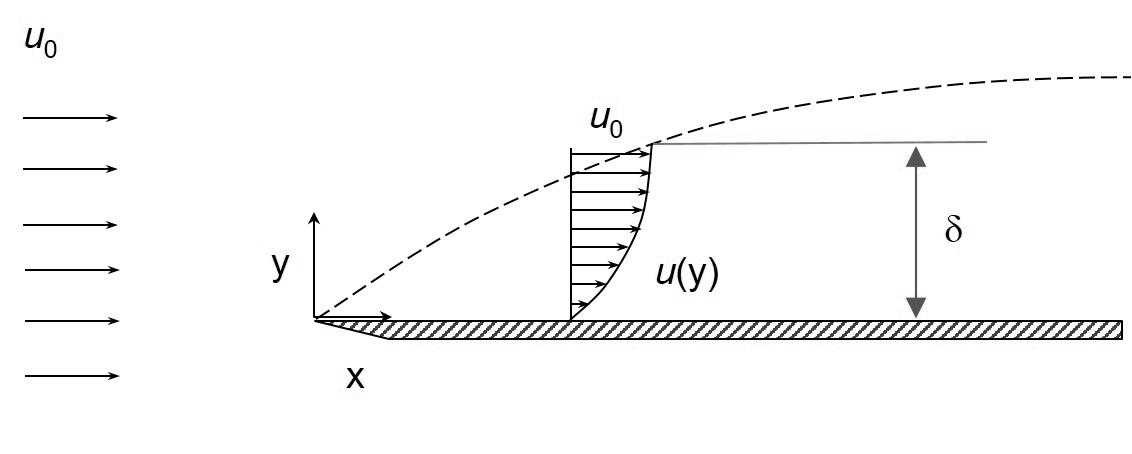
\includegraphics[width=0.6\linewidth]{../Assets/screenshot001}
		\caption{Пограничный слой}
		\label{fig:screenshot001}
	\end{figure}
	Чем меньше вязкость среды, тем тоньше гидродинамический пограничный слой и большее значение в этом слое имеет градиент скорости. Вне пограничного слоя градиент скорости невелик. Следовательно, силы трения здесь малы, и ими обычно пренебрегают. Между внешним потоком и пограничным слоем резкой границы нет, поскольку средняя скорость жидкости по сечению потока изменяется монотонно, без скачков. Обычно толщину пограничного слоя определяют условно, исходя из того, что на его внешней границе скорость составляет 99 \% от скорости внешнего потока.
	
	Значение пограничного слоя очень велико, так как он определяет гидродинамическое сопротивление при движении среды относительно твердого тела, а также сопротивление переносу массы и тепла. Введение этого понятия существенно упростило уравнения моделирования течение жидкости путём разделения потока на две области.
	
	В общем случае неизотермическое движение вязкой несжимаемой жидкости описывается следующими уравнениями: уравнения Навье-Стокса, уравнение несжимаемости, конвективной теплопроводности и состояния.
	\begin{align}
		& \frac{\partial u}{\partial t} + u\frac{\partial u}{\partial x} + v\frac{\partial u}{\partial y} + w\frac{\partial u}{\partial z} = -\frac{1}{\rho}\frac{\partial p}{\partial x} + \nu(\frac{\partial^2 u}{\partial x^2} + \frac{\partial^2 u}{\partial y^2} + \frac{\partial^2 u}{\partial z^2}) \nonumber\\
		& \frac{\partial v}{\partial t} + u\frac{\partial v}{\partial x} + v\frac{\partial v}{\partial y} + w\frac{\partial v}{\partial z} = -\frac{1}{\rho}\frac{\partial p}{\partial y} + \nu(\frac{\partial^2 v}{\partial x^2} + \frac{\partial^2 v}{\partial y^2} + \frac{\partial^2 v}{\partial z^2})\nonumber\\
		& \frac{\partial w}{\partial t} + u\frac{\partial w}{\partial x} + v\frac{\partial w}{\partial y} + w\frac{\partial w}{\partial z} = -\frac{1}{\rho}\frac{\partial p}{\partial z} + \nu(\frac{\partial^2 w}{\partial x^2} + \frac{\partial^2 w}{\partial y^2} + \frac{\partial^2 w}{\partial z^2})\nonumber\\
		& \frac{\partial u}{\partial x} + \frac{\partial v}{\partial y} + \frac{\partial w}{\partial z} = 0 \nonumber\\
		& \rho c (\frac{\partial T}{\partial\tau} + \vec{v}\nabla T) = div(\lambda \nabla T) + q_v + \mu\Phi - p div(\vec{v}) \nonumber\\
		& f(p, \rho, T) = 0
	\end{align}
	Исходя из этого имеем 6 уравнений и 6 неизвестных($u, v, w, \rho, T, p$). Эта система чрезвычайно сложна и в общем виде с трудом поддается решению даже современными численными методами на мощных компьютерах. Поэтому часто рассматривают различные упрощения этой системы.
	
	Существуют три вида течения в пограничном слое, каждое из которых имеет свои особенности и некоторые из них достаточны сложны для численного моделирования:
	\begin{itemize}
		\item ламинарное -- движение жидкости упорядочено, слои не смешиваются, частицы вращаются в пределах одного и того же тонкого слоя;
		\item турбулентное -- движение неупорядочено, происходит перемешивание частиц в поперечном направлении и весь пограничный слой беспорядочно завихрен;
		\item смешанное -- переходное состояние от ламинарного к турбулентному режиму движения.
	\end{itemize}
	В данной работе изучается турбулентный режим течения. Он является более сложным для численного моделирования.
\section{Турбулентное состояние пограничного слоя}
	Ламинарное течение устойчиво только при некоторых условиях, определяемых значением критического числа Рейнольдса $Re_{cr}$. Обычно переход от ламинарного к турбулентному режиму течения жидкости в трубах наблюдается при $Re_{cr} \approx 2300$. Турбулентное движение в пограничном слое возникает из-за нестабильности потока, которая проявляется в виде вихрей различных размеров и интенсивности. Эти вихри перемешивают слои жидкости, что приводит к увеличению переноса массы и энергии вдоль поверхности твердого тела. Турбулентное течение с большим числом Рейнольдса называют развитой турбулентностью.
	
	На значение критического числа можно влиять. Если вход в трубу сделать плавным, то ламинарное движение в трубе может поддерживаться при больших числах Рейнольдса, например до 24000. Существенно влияют на $Re_{cr}$ и такие факторы, как градиент давления, форма канала, шероховатость его стенок, вдув и откачка пограничного слоя. Возрастание давления в направлении движения приводит к неустойчивости течения в пограничном слое, отрыву и возникновению вихрей. Поэтому как для внутренних (в трубах и каналах), так и для внешних (обтекание тел потоком) течений критическое число Рейнольдса возрастает при уменьшении внешнего градиента давления (ускоряющиеся течения -- по закону Бернулли).
	\begin{figure}[H]
		\centering
		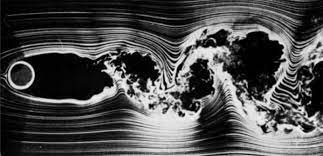
\includegraphics[width=0.7\linewidth]{../Assets/turb}
		\caption{Пример турбулентности}
		\label{fig:turb}
	\end{figure}

	Турбулентность можно определить как трехмерное нестационарное движение, в котором вследствие растяжения вихрей создается непрерывное распределение пульсаций скорости в интервале длин волн от минимальных, определяемых вязкими силами, до максимальных, определяемых граничным условиями течения. При математическом описании турбулентных течений удобно исходить из понимания турбулентности как иерархии вихрей различного масштаба, используя вихревую и волновую трактовку турбулентности\cite{Монин1992}. Турбулентные вихри непрерывны и постоянно соприкасаются друг с другом, причем крупные вихри, размеры которых определяются граничными условиями задачи, содержат в себе вихри меньших размеров.
	
	Максимальный размер вихрей близок к характерному линейному масштабу задачи $L$. Часто движение наиболее крупных вихрей оказывается в значительной степени упорядоченным (например, течение за цилиндром). Такие структуры называют когерентными. Вихри минимального размера диссипируют непосредственно в тепло. Их размер характеризуется колмогоровским масштабом $\eta_k = (\nu^3/\epsilon)^{1/4}$. Наибольшее количество энергии при этом переносят вихри некоторого среднего размера.
	
	Одной из важных характеристик описывающих турбулентное движение это завихрённость $\omega$: 
	\begin{align}
		\vec{\omega} = \vec{\nabla}\times \vec{v} \qquad \omega_x = \frac{\partial w}{\partial y} - \frac{\partial v}{\partial z}, \qquad \omega_y = \frac{\partial u}{\partial z} - \frac{\partial w}{\partial x}, \qquad \omega_z = \frac{\partial v}{\partial x} - \frac{\partial u}{\partial y}
	\end{align}

\section{Структура пограничного слоя}
	Представления о структуре профиля скорости постепенно менялись и окончательно сформировались к концу 1950х годов. В турбулентном пограничном слое обычно выделяется две области: внешняя и внутрення. Они отличаются друг от друга разными масштабами вихревых структур\cite{Белов2001}.
	\begin{figure}[H]
		\centering
		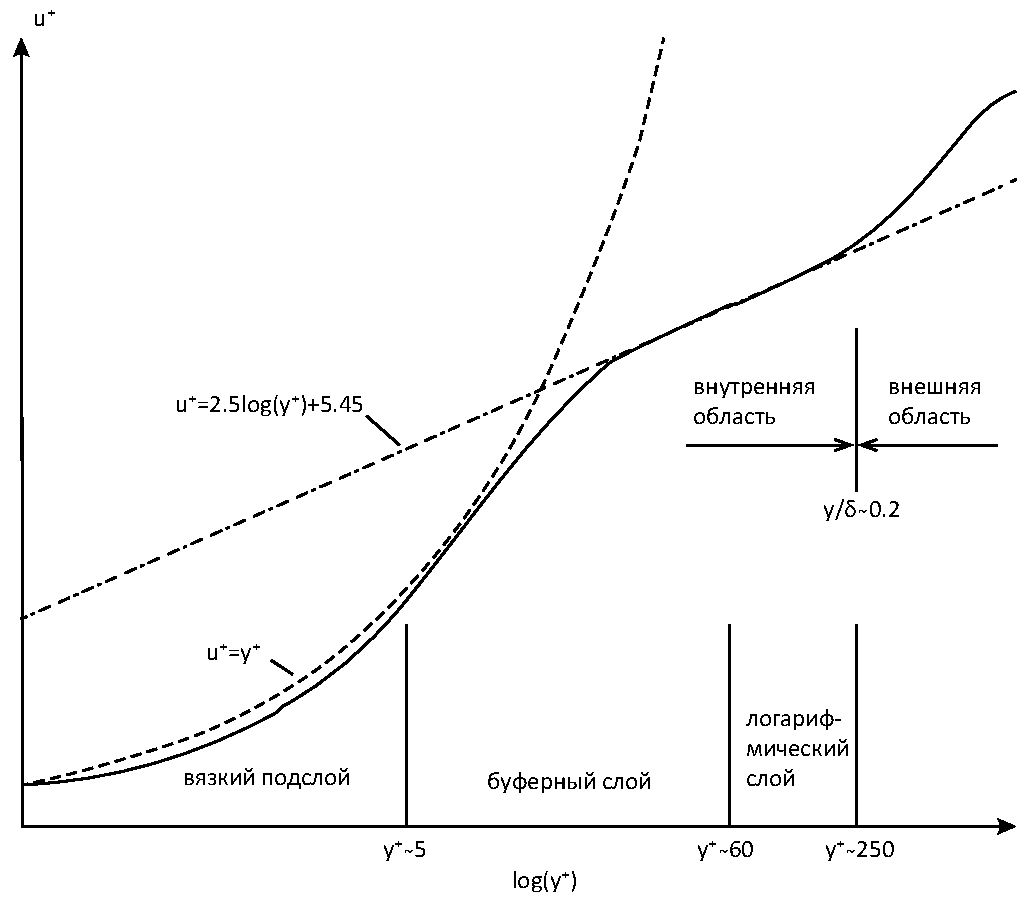
\includegraphics[width=0.6\linewidth]{../Assets/ПогранСлойRU}
		\caption{Схема слоя}
	\end{figure}
	Внутренняя область пограничного слоя занимает примерно 20\% от толщины всего слоя и в ней генерируется до 80\% энергии турбулентности. На формирование течения в пограничном слое основное влияние оказывают вязкость, теплопроводность и диффузионная способность жидкости. Внутри динамического пограничного слоя происходит плавное изменение скорости от её значения во внешнем потоке до нуля на стенке вследствие прилипания вязкой жидкости к твёрдой поверхности. Аналогично внутри пограничного слоя плавно изменяется температура.
			
\subsection{Внешняя область}

	Внешний слой является областью полностью развитого турбулентного течения, в котором распределение скорости описывается логарифмическим законом. Полное затухание возмущений во внешней области происходит на расстоянии, во много раз превышающем линейный масштаб турбулентности.
	
	Чтобы определить поток во внешней зоне, применяют фильтрованные или осредненные по Рейнольдсу уравнения Навье-Стокса. В то же время, профиль скорости во внутренней зоне сравнительно мало зависит от различных внешних условий, таких как числа Рейнольдса и градиент давления, что позволяет использовать универсальные соотношения (пристеночные функции) для связи параметров потока с расстоянием от стенки. Этот метод также базируется на гипотезе о локальном равновесии энергии турбулентных пульсаций и свойствах локальной изотропности диссипирующих вихрей\cite{Волков2005}.

\subsection{Внутренняя область}

	Вязкий подслой, буферный и логарифмический слои составляют внутреннюю область пограничного слоя. Она характеризуется высокой скоростью переноса массы, импульса и тепла, что приводит к повышенной трению и потере энергии.
	\begin{align}
		v\frac{\partial u}{\partial y} \gg -\overline{u'v'} & \qquad\text{вязкий}\nonumber \\
		v\frac{\partial u}{\partial y} \approx -\overline{u'v'} & \qquad\text{буферный}\nonumber \\
		v\frac{\partial u}{\partial y} \ll -\overline{u'v'} & \qquad\text{логарифмический}
	\end{align}
	
	Существует два подхода к моделированию течения в пристеночной области. В первом подходе используются полуэмпирические формулы (пристеночные функции) для описания внутреннего слоя потока, в то время как во втором подходе модели турбулентности модифицируются таким образом, чтобы разрешать всю пристеночную область потока, включая вязкий подслой, при условии обеспечения необходимого разрешения сетки в пограничном слое. Такие модели турбулентности могут быть использованы для расчета турбулентных течений во всей расчетной области (включая пристеночную область течения).

\subsection{Свойства пограничного слоя}
	
	Толщина пограничного слоя трудно определима как в расчёте, так и в эксперименте. Для определения используются понятия: толщина вытеснения $\delta^*$ и толщина потери импульса $\theta$.
	\begin{equation}
		\delta^* = \int_{0}^{\infty}(1 - \frac{u}{U_0})dy \qquad \theta = \delta^{**} = \int_{0}^{\infty} \frac{u}{U_0}(1 - \frac{u}{U_0})dy
	\end{equation}
	Кроме того используется безразмерный параметр $H$:
	\begin{equation}
		H = \frac{\delta^*}{\theta}
	\end{equation}
	
	Число Рейнольдса характеризуется двумя величинами($Re_x$ и $Re_\theta$): расстоянием от нижней стенки $x$ и толщиной $\theta$.
	\begin{equation}
		Re_x = \frac{xU_0}{\nu} \qquad Re_\theta = \frac{\theta U_0}{\nu}
	\end{equation}
	
	Используя напряжение трения на стенке $\tau_w$ можем вычислить коэффициент трения $C_F$ и динамическую скорость $u_\tau$:
	\begin{equation}
		\tau_w = \nu\frac{\partial u}{\partial y}\bigg|_W \qquad C_F = \frac{\tau_w}{0.5\rho U_0^2} \qquad u_\tau = \sqrt{\frac{\tau_w}{\rho}}
	\end{equation}
	
	Не менее важной характеристикой пограничных слоев является продольный градиент давления:
	\begin{equation}
		\frac{dp}{dx} = -\rho U_0 \frac{dU_0}{dx}
	\end{equation}
	
	Часто на пограничные слои влияют такие факторы: кривизна поверхности $\kappa$, скорость закачки и откачки жидкости, шероховатость поверхности $k_s^+$(высота бугорков).
	\begin{equation}
		\kappa = \frac{\delta^*}{R} \qquad \frac{V_W}{u_\tau}, \frac{V_W}{U_0} \qquad k_s^+ = \frac{k_s u_\tau}{\nu}
	\end{equation}
	
	Важным свойством пограничного слоя является выполнение интегрального уравнения импульсов. Верно и обратное: если уравнение импульсов не выполняется, то уравнения плоского пограничного слоя также не верны для этого течения. Это может быть обусловлено разными причинами: трехмерность течения, его нестационарность, влияние вверх по потоку, изменение давления поперек пограничного слоя, влияние нормальных Рейнольдсовых напряжений и т.д.
	\begin{equation}
		\frac{d\theta}{dx} + \frac{dU_0}{dx}\cdot\frac{2 + H}{U_0}\theta - \frac{C_f}{2} = 0
	\end{equation}

\subsection{Закон стенки}
	
	Для работы с пограничным слоем обычно используются безразмерные параметры $u^+$ и $y^+$:
	\begin{equation}
		u^+ = \frac{u}{u_\tau} \qquad y^+ = \frac{yu_\tau}{v}
	\end{equation}
	В вязком подслое вязкие напряжения намного больше над рейнольдсовыми, а скорость линейно зависит от расстояния до стенки. В буферном слое напряжения имеют одинаковый порядок. В логарифмическом слое рейнольдсовы напряжения намного превышают вязкие напряжения, а профиль скорости описывается логарифмическим законом.
	\begin{align}
		&u^+ = y^+ & 0 \leq y^+ < 5 & \qquad\text{вязкий} \nonumber\\
		&u^+ \neq y^+ & 5 \leq y^+ < 60 & \qquad\text{буферный} \nonumber\\
		&u^+ = \frac{1}{Ka}ln E y^+ & 60 \leq y^+ < 0.2\delta & \qquad\text{логарифмический}
	\end{align}
	В данном случае число Кармана $Ka$ и параметр $E$, который зависит от шероховатости поверхности, определяются на основе экспериментальных данных. 
	\begin{equation}
		Ka = \frac{1}{u}\sqrt{\frac{R_x^2 + R_y^2 + R_z^2}{3}}
	\end{equation}

	Закон стенки можно рассматривать как решение уравнений движения в турбулентном пограничном слое, полученное при использовании модели пути смешения Прандтля. Обычно считается, что закон стенки выполняется при $30 < y^+ < 200$. Конкретная реализация подхода зависит от выбранной модели турбулентности и используемой разностной схемы. Функции, входящие в закон стенки, нуждаются в модификации для точного описания эффектов, связанных с возможной шероховатостью поверхности. Закон стенки трудно приспособить для расчета течений со сложной геометрией на неструктурированных сетках.

\section{Методы моделирования}
	
	Несмотря на интенсивное развитие вычислительной техники и впечатляющие успехи, достигнутые в последние годы как в области построения эффективных численных алгоритмов, предназначенных для решения задач гидромеханики и тепломассопереноса, так и в разработке сопутствующего математического обеспечения (генераторы сеток, интерактивные системы ввода данных и систем визуализации результатов расчетов), проблема численного моделирования турбулентности, как и на протяжении многих предшествующих десятилетий, по-прежнему остается одной из наиболее сложных и актуальных проблем механики жидкостей. В отличие от ламинарных течений однофазной среды (жидкости), расчет которых, благодаря отмеченным выше достижениям, стал во многом рутинной процедурой, надежное предсказание характеристик сложных турбулентных течений, представляющих наибольший практический интерес все еще остается сложным.
	\begin{figure}[H]
		\centering
		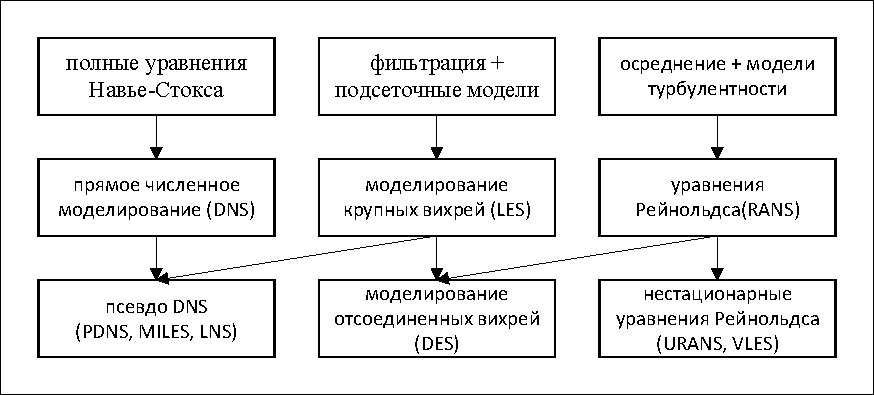
\includegraphics[width=0.9\linewidth]{../Assets/СхемаМетодовRU}
		\caption{Виды методов по уравнениям}
		\label{fig:cheme}
	\end{figure}
	
	Среди основных методов численного моделирования трехмерных турбулентных течений можно выделить: прямое численное моделирование (DNS), моделирование крупных вихрей (LES) и решение осредненных по Рейнольдсу уравнений Навье-Стокса (RANS). Имеются также различные промежуточные подходы, сочетающие в себе те или иные черты RANS, LES и DNS, например, метод моделирования отсоединенных вихрей (DES), и ряд других, не имеющих должного физического обоснования и потому не получивших широкого распространения.

\subsection{DNS}
	
	Прямое численное моделирование(DNS) предполагает решение полных нестационарных трехмерных уравнений Навье-Стокса, позволяющее получить мгновенные характеристики турбулентного потока. Проблемы с широким использованием DNS связаны с высокими требованиями к используемой разностной схеме, удовлетворением начальных и граничных условий, а также ограниченными ресурсами вычислительной техники. Расчетная область при этом должна быть достаточно протяженной, чтобы вместить наибольшие масштабы турбулентности, а шаг интегрирования по времени должен иметь порядок колмогоровского масштаба.
	
	\begin{table}[H]
		\begin{center}
			\begin{tabular}{|c|c|c|c|c|}
				\hline
				Re & 6.6$\times10^3$ & 2.0$\times10^4$ & 1.0$\times10^5$ & 1.0$\times10^6$\\
				\hline
				Кол-во узлов сетки & 2$\times10^6$ & 4$\times10^7$ & 3$\times10^8$ & 1.5$\times10^3$\\
				\hline
				150 MFlops & 37 ч & 740 ч & 6.5 лет & 3000 лет\\
				\hline
				1 TFlops & 20 с & 400 с & 8.3 ч & 4000 ч\\
				\hline
			\end{tabular}
		\end{center}
		\caption{Затраты времени при различных параметрах}
	\end{table}

	Эти жесткие требования отчасти смягчаются при использовании высокоточных спектральных методов численного интегрирования уравнений Навье-Стокса, которые	часто используются для DNS. Однако эти методы неприменимы к расчету течений со сложной геометрией. Указанные обстоятельства приводят к тому, что на практике DNS применяется только для расчета простых турбулентных течений при низких числах Рейнольдса. При этом основной задачей расчета является не	собственно получение данных о характеристиках осредненного течения (они, как правило, известны), а получение детальной информации о структуре турбулентности, а также вычисление отдельных членов, входящих в те или иные модели турбулентности.

\subsection{RANS}
	
	В инженерных приложениях широко используются математические модели, основанные на численном решении осредненных по Рейнольдсу уравнений Навье-Стокса(RANS). При использовании уравнений Рейнольдса основной интерес проявляется к динамике крупномасштабных вихрей, ответственных за переносные свойства турбулентных течений. При замыкании уравнений Рейнольдса рассматриваются масштабы длины, типичные для энергосодержащих вихрей, в которых $Re\gg1$ (за исключением пристеночных областей). Для учета пристеночного влияния диссипирующих вихрей и энергосодержащих вихрей при $Re\sim1$ используются демпфирующие функции. Применив к уравнениям осреднение Рейнольдса получим:
	\begin{align}
				&\frac{\partial u_i}{\partial x_i} = 0 \nonumber\\
				&\rho\frac{\partial u_i}{\partial t} + \rho u_j \frac{\partial u_i}{\partial x_j} = - \frac{\partial p}{\partial x_i} + \frac{\partial}{\partial x_j}(\mu\frac{\partial u_i}{\partial x_j} - \rho\overline{u_i' u_j'})
	\end{align}

	Эта система является незамкнутой, поскольку в нее входит неизвестный тензор так называемых рейнольдсовых напряжений $\tau_{ij} = -\rho\overline{u_i' u_j'}$(турбулентные напряжения). Для замыкания этой системы уравнений необходимо определить шесть различных компонент симметричного тензора турбулентных напряжений. Именно выражение этих компонент через параметры осредненного потока и называется моделью турбулентности. Ниже представлена таблица с основными этапами развития теории.
	
	\begin{table}[H]
		\begin{center}
			\begin{tabular}{|c|c|c|}
				\hline
				Год & Ученые & Что изучено\\
				\hline
				1877 & Буссинеск Ж. В. & гипотеза Буссинеска\\
				\hline
				1895 & Рейнольдс О. & осреднение по Рейнольдсу\\
				\hline
				1925 & Прандтль Л. & теория пути смешивания Прандтля\\
				\hline
				1930 & Карман Т. & формула Кармана\\
				\hline
				1942 & Колмогоров А. Н. & формула Колмогорова, модель $k$-$\omega$\\
				\hline
				1951 & Ротта & первая модель Рейнольдсовых напряжений\\
				\hline
				1956 & Клаузер & формула Клаузера\\
				\hline
				1956 & Ван-Дрист & демпфирующий множитель\\
				\hline
				1974 & Лондер Б. и Сполдинг Д. & модель $k$-$\epsilon$\\
				\hline
			\end{tabular}
		\end{center}
		\caption{Этапы развития теории}
	\end{table}
	
	Появление огромного количества моделей привело к необходимости выбора. Для этого необходимо провести сравнительный анализ моделей. Однако при попытке тестирования естественным образом возникают определенные трудности. Во-первых, необходимо выбрать течения, для которых известен набор достоверных экспериментальных данных, свободных от погрешностей, а также выбрать критерии для сравнения моделей. Во-вторых, необходимо провести серийные расчеты этих течений с использованием разных моделей турбулентности и при этом быть уверенными в независимости результата от программной реализации задачи. Результатом такой работы должны явиться рекомендации по области применимости тех или иных моделей турбулентности.

\subsection{LES}
	
	Метод моделирования крупных вихрей(LES) был предложен Иосифом Смагоринским в 1963 году. Он основан на двух предположениях. Первый предполагает, что течение можно разделить на движение крупных и мелких вихрей. Крупные вихри, находящиеся под прямым воздействием граничных условий и несущие в себе максимум рейнольдсовых напряжений, рассчитываются. Мелкомасштабная турбулентность считается изотропной и имеющей универсальные характеристики, а потому менее критичной и более поддающейся моделированию. Другой  заключается в возможности аппроксимации нелинейных взаимодействий между крупными и мелкими вихрями только по крупным вихрям с использованием подсеточных моделей(SGS). Иначе говоря, принимается гипотеза о статистической независимости крупных и мелких вихрей.
	
	Статистика крупных вихрей обычно не чувствительна к подсеточному моделированию за исключением пристеночной области. Имеющиеся подсеточные модели корректно предсказывают не только осредненные характеристики потока (первые и вторые моменты), но также и флуктуации интегральных характеристик, например, коэффициентов сопротивления и подъемной силы\cite{Fureby2000}.
	
	Мелкомасштабное движение исключается из уравнений Навье-Стокса при помощи применения операции фильтрации и моделируются с помощью подсеточных моделей. На рисунке \ref{fig:lesfilter} показан принцип работы фильтров, где $g(x)$ - исходный вариант, $f(x)$ - после фильтрации.\\
	\begin{figure}[H]
		\centering
		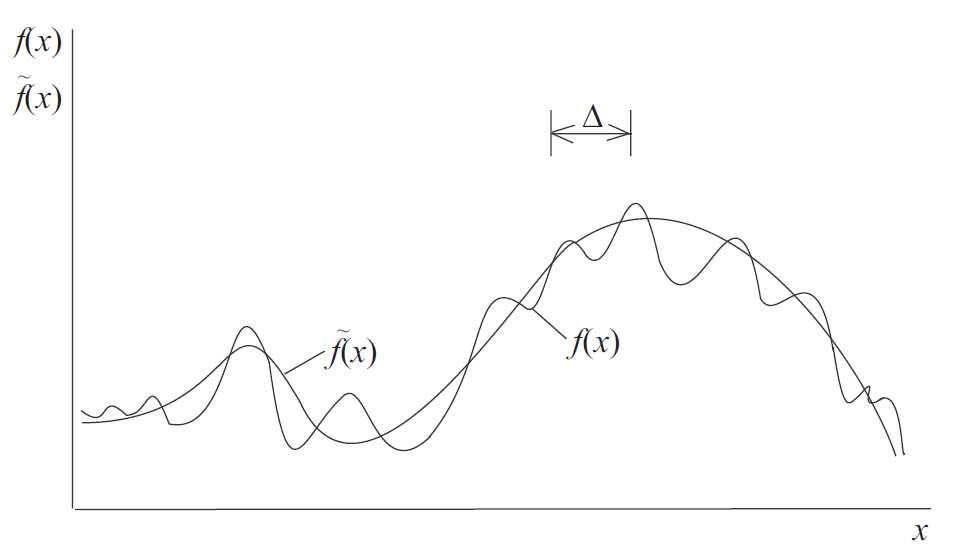
\includegraphics[width=0.7\linewidth]{../Assets/ФильтрацияLES}
		\caption{Исключение мелкомасштабных движений фильтрацией}
		\label{fig:lesfilter}
	\end{figure}
	Уравнение фильтра, применимое к пространственно временному полю $\phi(x,t)$ представлено ниже:
	\begin{equation}
		\overline{\phi(x,t)} = \int_{-\infty}^{\infty}\int_{-\infty}^{\infty}\phi(r,t')G(x - r, t - t')dt'dr
	\end{equation}
	В данном случае $G$ - ядро, характерное для каждого типа фильтра.
	
	Решение, полученное с помощью LES, содержит более богатую информацию по сравнению с решением на основе уравнений Рейнольдса, например, не только характеристики среднего течения (поля скорости, концентрации, температуры, давления) и распределения рейнольдсовых напряжений, но также и спектральные характеристики (спектры пульсаций скорости и давления), двухточечные моменты, временные и пространственные масштабы турбулентности.

\subsection{DES}
	
	Характерные для отрывных течений крупномасштабные нестационарные трехмерные вихревые структуры определяются конкретными граничными условиями и геометрическими характеристиками рассматриваемых течений и не могут быть описаны в рамках таких моделей. Это стимулируют поиск и разработку гибридных подходов, сочетающих в себе экономичность RANS и универсальность LES.
	
	В методе моделирования отсоединенных вихрей (DES) в области присоединенного пограничного слоя метод функционирует в режиме уравнений Рейнольдса, а в области отрыва потока переходит в LES. При этом достигается сочетание лучших качеств обоих подходов -- высокая точность и экономичность уравнений Рейнольдса в области присоединенного пограничного слоя и универсальность LES в отрывной области. Хотя DES, в отличие от RANS, является принципиально нестационарным трехмерным подходом, необходимые для его реализации сетки в пристеночной области совпадают с сетками, необходимыми для решения уравнений Рейнольдса, и являются на много порядков меньшими, чем сетки, требуемые для разрешения мелких пристенных вихрей в рамках LES. По мере измельчения сетки DES асимптотически приближается к LES и далее к DNS. Конкретные реализации DES основаны на использовании модели турбулентной вязкости Спаларта-Аллмараса и модели Ментера\cite{Strelets2001}.
	
	Как следует из названия метода DES, он создавался для расчета отрывных течений. Такие течения лучше подходят для этого метода. Во-первых, наличие массированного отрыва в большинстве случаев приводит к его пульсациям, как следствие этого, к возникновению автоколебательного течения с крупными когерентными структурами. Во-вторых, наличие отрывной зоны позволяет обойти проблему создания турбулентных пульсаций на входе в LES области.
	
\subsection{PDF}
	Функция плотности вероятности для турбулентных режимов была введена Лундгреном в 1969 году\cite{Lundgren1969}. Этот подход аналогичен кинетической теории газов, в которой макроскопические свойства газа описываются большим числом частиц. Методы PDF уникальны тем, что они могут применяться в рамках ряда различных моделей турбулентности; основные различия встречаются в форме уравнения переноса PDF. Например, в контексте метода крупных вихрей PDF становится фильтрованным и приводит к уравнению Ланжевена.
	\begin{figure}[H]
		\centering
		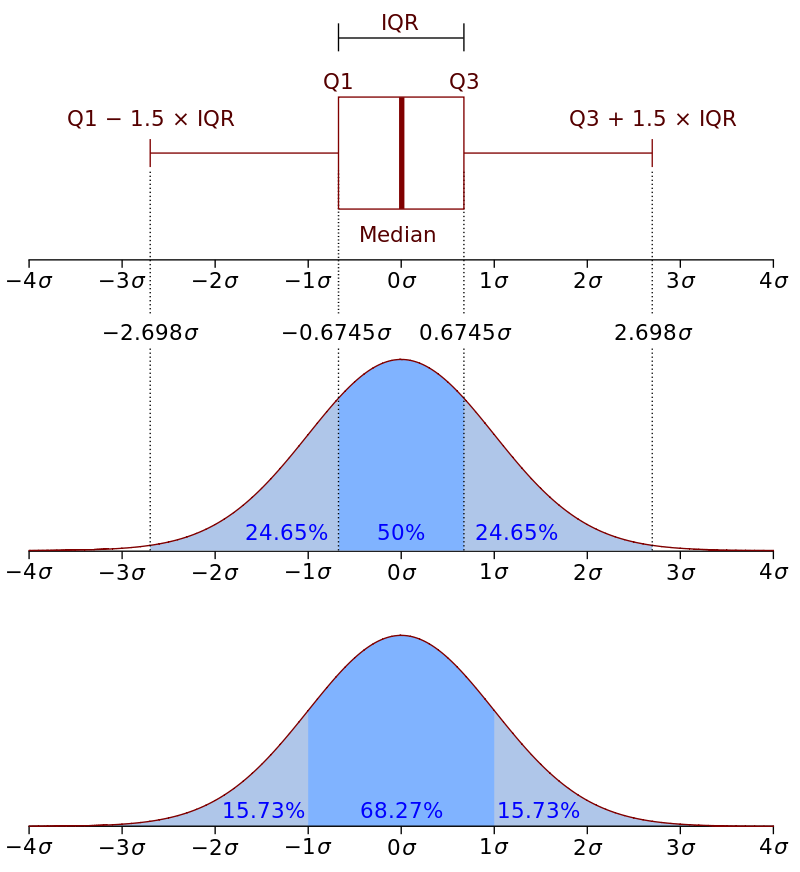
\includegraphics[width=0.7\linewidth]{../Assets/pdfplot}
		\caption{Функция плотности вероятности нормального распределения}
		\label{fig:pdfplot}
	\end{figure}
	В более точном смысле PDF используется для определения вероятности того, что случайная величина попадет в определенный диапазон значений, а не примет какое-либо одно значение. Эта вероятность определяется интегралом PDF этой переменной в этом диапазоне, то есть она определяется площадью под функцией плотности между самым низким и самым большим значениями диапазона. Функция плотности вероятности всюду неотрицательна, а площадь под всей кривой равна 1.
\subsection{Оценка производительности}
	
	Оценка количества узлов сетки и временных шагов, необходимых для реализации DNS и LES, показывает сложность проблемы с вычислительной точки зрения.
	
	\begin{table}[H]
		\begin{center}
			\begin{tabular}{|c|c|c|c|c|}
				\hline
				Метод & Число узлов сетки & Число шагов по времени & Готовность\\
				\hline
				RANS & $10^7$ & $10^3$ & 1985\\
				\hline
				DES & $10^8$ & $10^4$ & 2000\\
				\hline
				LES & $10^{11.5}$ & $10^{6.7}$ & 2045\\
				\hline
				DNS & $10^{16}$ & $10^{7.7}$ & 2080\\
				\hline
			\end{tabular}
		\end{center}
		\caption{Перспектива применения методов}
	\end{table}
	Готовность означает практическое применение метода с затратой времени не более суток.
	Для оценки необходимых вычислительных ресурсов (например, быстродействия и объема оперативной памяти) возьмем расчетную сетку 100$\times$100$\times$100 узлов($10^6$ точек). В каждом узле необходимо вычислить около 10 функций (составляющие скорости, плотность, давление, температуру, характеристики турбулентности, концентрации компонентов смеси). Значения неизвестных функций находятся в результате решения системы нелинейных уравнений, что требует от 200 до 1000 арифметических операций. За один шаг по времени необходимо выполнить $10^{10}$ операций с плавающей точкой. Для исследования развития процесса во времени требуется до 1000 временных шагов. В результате, выполнение одного расчета требует $10^{13}$ операций с плавающей точкой. Для проведения одного расчетного варианта компьютер с производительностью 100 МФлопc($10^8$ операций с плавающей точкой в секунду) затратит $10^7$ секунд. Для проведения расчета за 100 минут потребуется компьютер с производительностью 0.1 ТФлопс.